% !TeX encoding = UTF-8
% !TeX root = V30_Nonlinear.tex
% !TeX spellcheck = en_US

\section{Introduction}

\section{Theory}

\subsection{Laser diode}


\subsection{Nd:YAG laser}
The laser is based on a Nd:YAG crystal (yttrium aluminium garnet doped with neodymium).

For our laser, the \textsf{Nd} atoms can be approximated as a 4 level system:
\begin{itemize}
\item 1 $\rightarrow$ 4 : Absorption of red light around 805\,nm from the laser diode
\item 4 $\rightarrow$ 3 : Decay into state 3
\item 3 $\rightarrow$ 2 : Emission of infrared light at 1064\,nm
\item 2 $\rightarrow$ 1 : Decay into state 1
\end{itemize}


As the decays are nearly instantaneous, only states 1 and 3 are populated:
\begin{equation}
n_2 \approx n_4 \approx 0
\end{equation}

\begin{figure}[h]
	\centering
	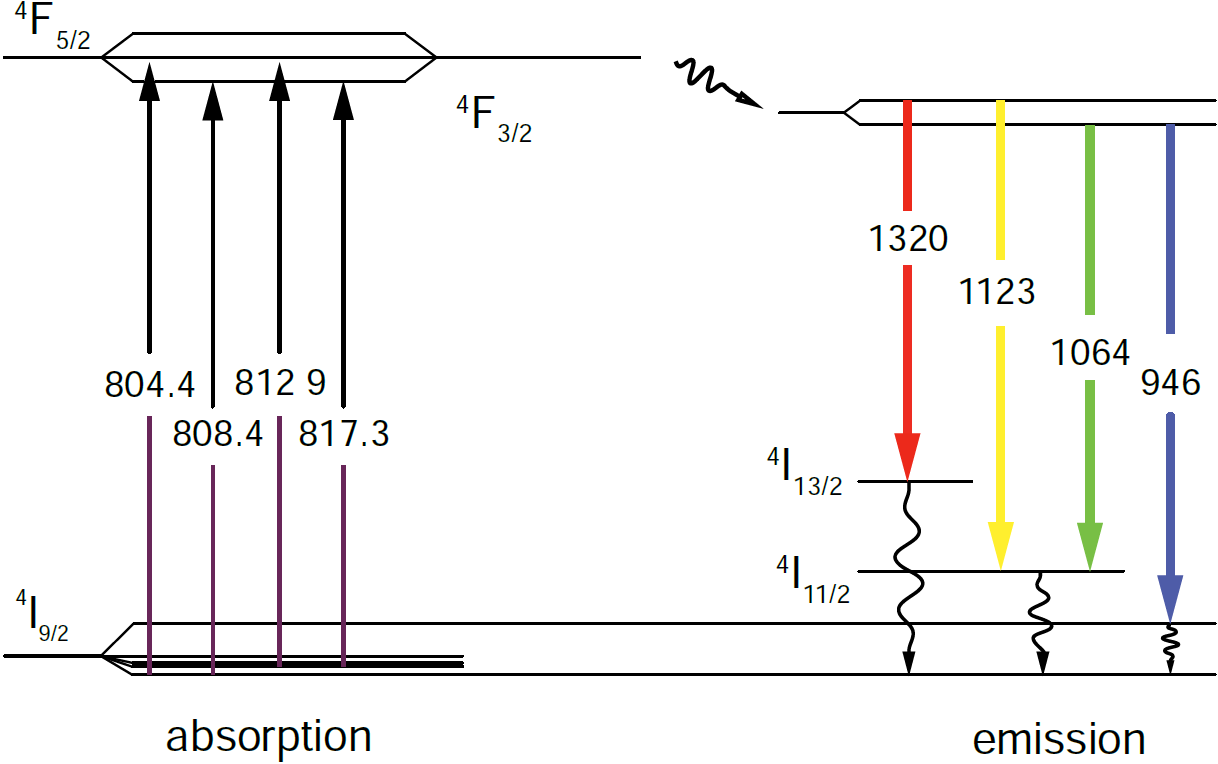
\includegraphics[width=\textwidth]{spectrum.png}
	\caption{Transitions in the Nd:YAG crystal \cite{lit:leybold}.}
	\label{fig:spectrum}
\end{figure}


\subsection{Nonlinear effect}
KTP crystal (Potassium titanyl phosphate, $\mathsf{K\,TiO\,PO_4}$)

two photon effect, quadratic

frequency doubling

energy conservation: $E = h \nu$
\begin{equation}
	\nu_2 = 2 \nu_1
\end{equation}

momentum conservation: $\vec p = \hbar \vec k$
\begin{equation}
	\vec k_2 = 2 \vec k_1
\end{equation}

$k = \frac{2 \pi}{\lambda}$
dispersion relation: $c = n c_0 = \lambda \nu$
\begin{equation}
2 = \frac{k_2}{k_1} = \frac{n_2 \nu_2}{n_1 \nu_1} = 2\;\frac{n_2}{n_1}
\end{equation}

Thus the refraction index of the material has to be the same for both wavelengths. As most materials show normal diffraction, i.e. $n(\lambda) \searrow$, 
